\documentclass[12pt]{exam}
%\documentclass[12pt]{article}
\usepackage[letterpaper, margin=0.75in]{geometry}
\usepackage{graphicx}
\usepackage{enumitem}
\usepackage{booktabs}
\usepackage{amsmath}
\usepackage{tabularx}

\begin{document}
\footer{}{Page \thepage\ of \numpages}{}

\begin{flushright}
\makebox[0.5\textwidth]{\large Name:\enspace\hrulefill}
\vspace{0.2in}

\makebox[0.5\textwidth]{\large Date:\enspace\hrulefill}
\end{flushright}

\begin{center}

\includegraphics[width=10cm]{../images/logo.png}
\end{center}

\begin{center}
\noindent{\LARGE Conceptual Physics \\ Class 2 Questions \\ Feb 9, 2018 \\}
\end{center}
\vspace{0.2in}


\vspace{0.2in}

The following table of metric prefixes may be useful:
\vspace{0.2in}

\noindent\begin{tabularx}{\textwidth}{ X X X X X X }
	kilo & (none) & centi & mili & micro & nano \\
	k & (none) & c & m & $\mu$ & n \\
	$10^3$ & $10^0$ & $10^{-2}$ & $10^{-3}$ & $10^{-6}$ & $10^{-9}$ \\
	1000 & 1 & 0.01 & 0.001 & 0.000001 & 0.000000001 
\end{tabularx}

\clearpage

\begin{questions}

\question
You are the manager for a landscaping company, and are comparing 3 different materials suppliers. Each sells the same material, only packaged differently. Your job is to compare the different sellers, and in particular look at how they package sand.

\begin{itemize}
\item Supplier 1 sells sand in \textit{buckets}.
\item Supplier 2 sells sand in \textit{bags}. 
\item Supplier 3 sells sand in \textit{crates}.
\end{itemize}

Although each supplier packages sand differently, you find out that 1~bag can be split into 10~buckets, and that 10~bags fill 1~crate.

\noindent\begin{tabularx}{\textwidth}{ X | X | X }
	Supplier 1 sells sand in \textit{buckets} & Supplier 2 sells sand in \textit{bags} & Seller 3 sells sand in \textit{crates} \\
	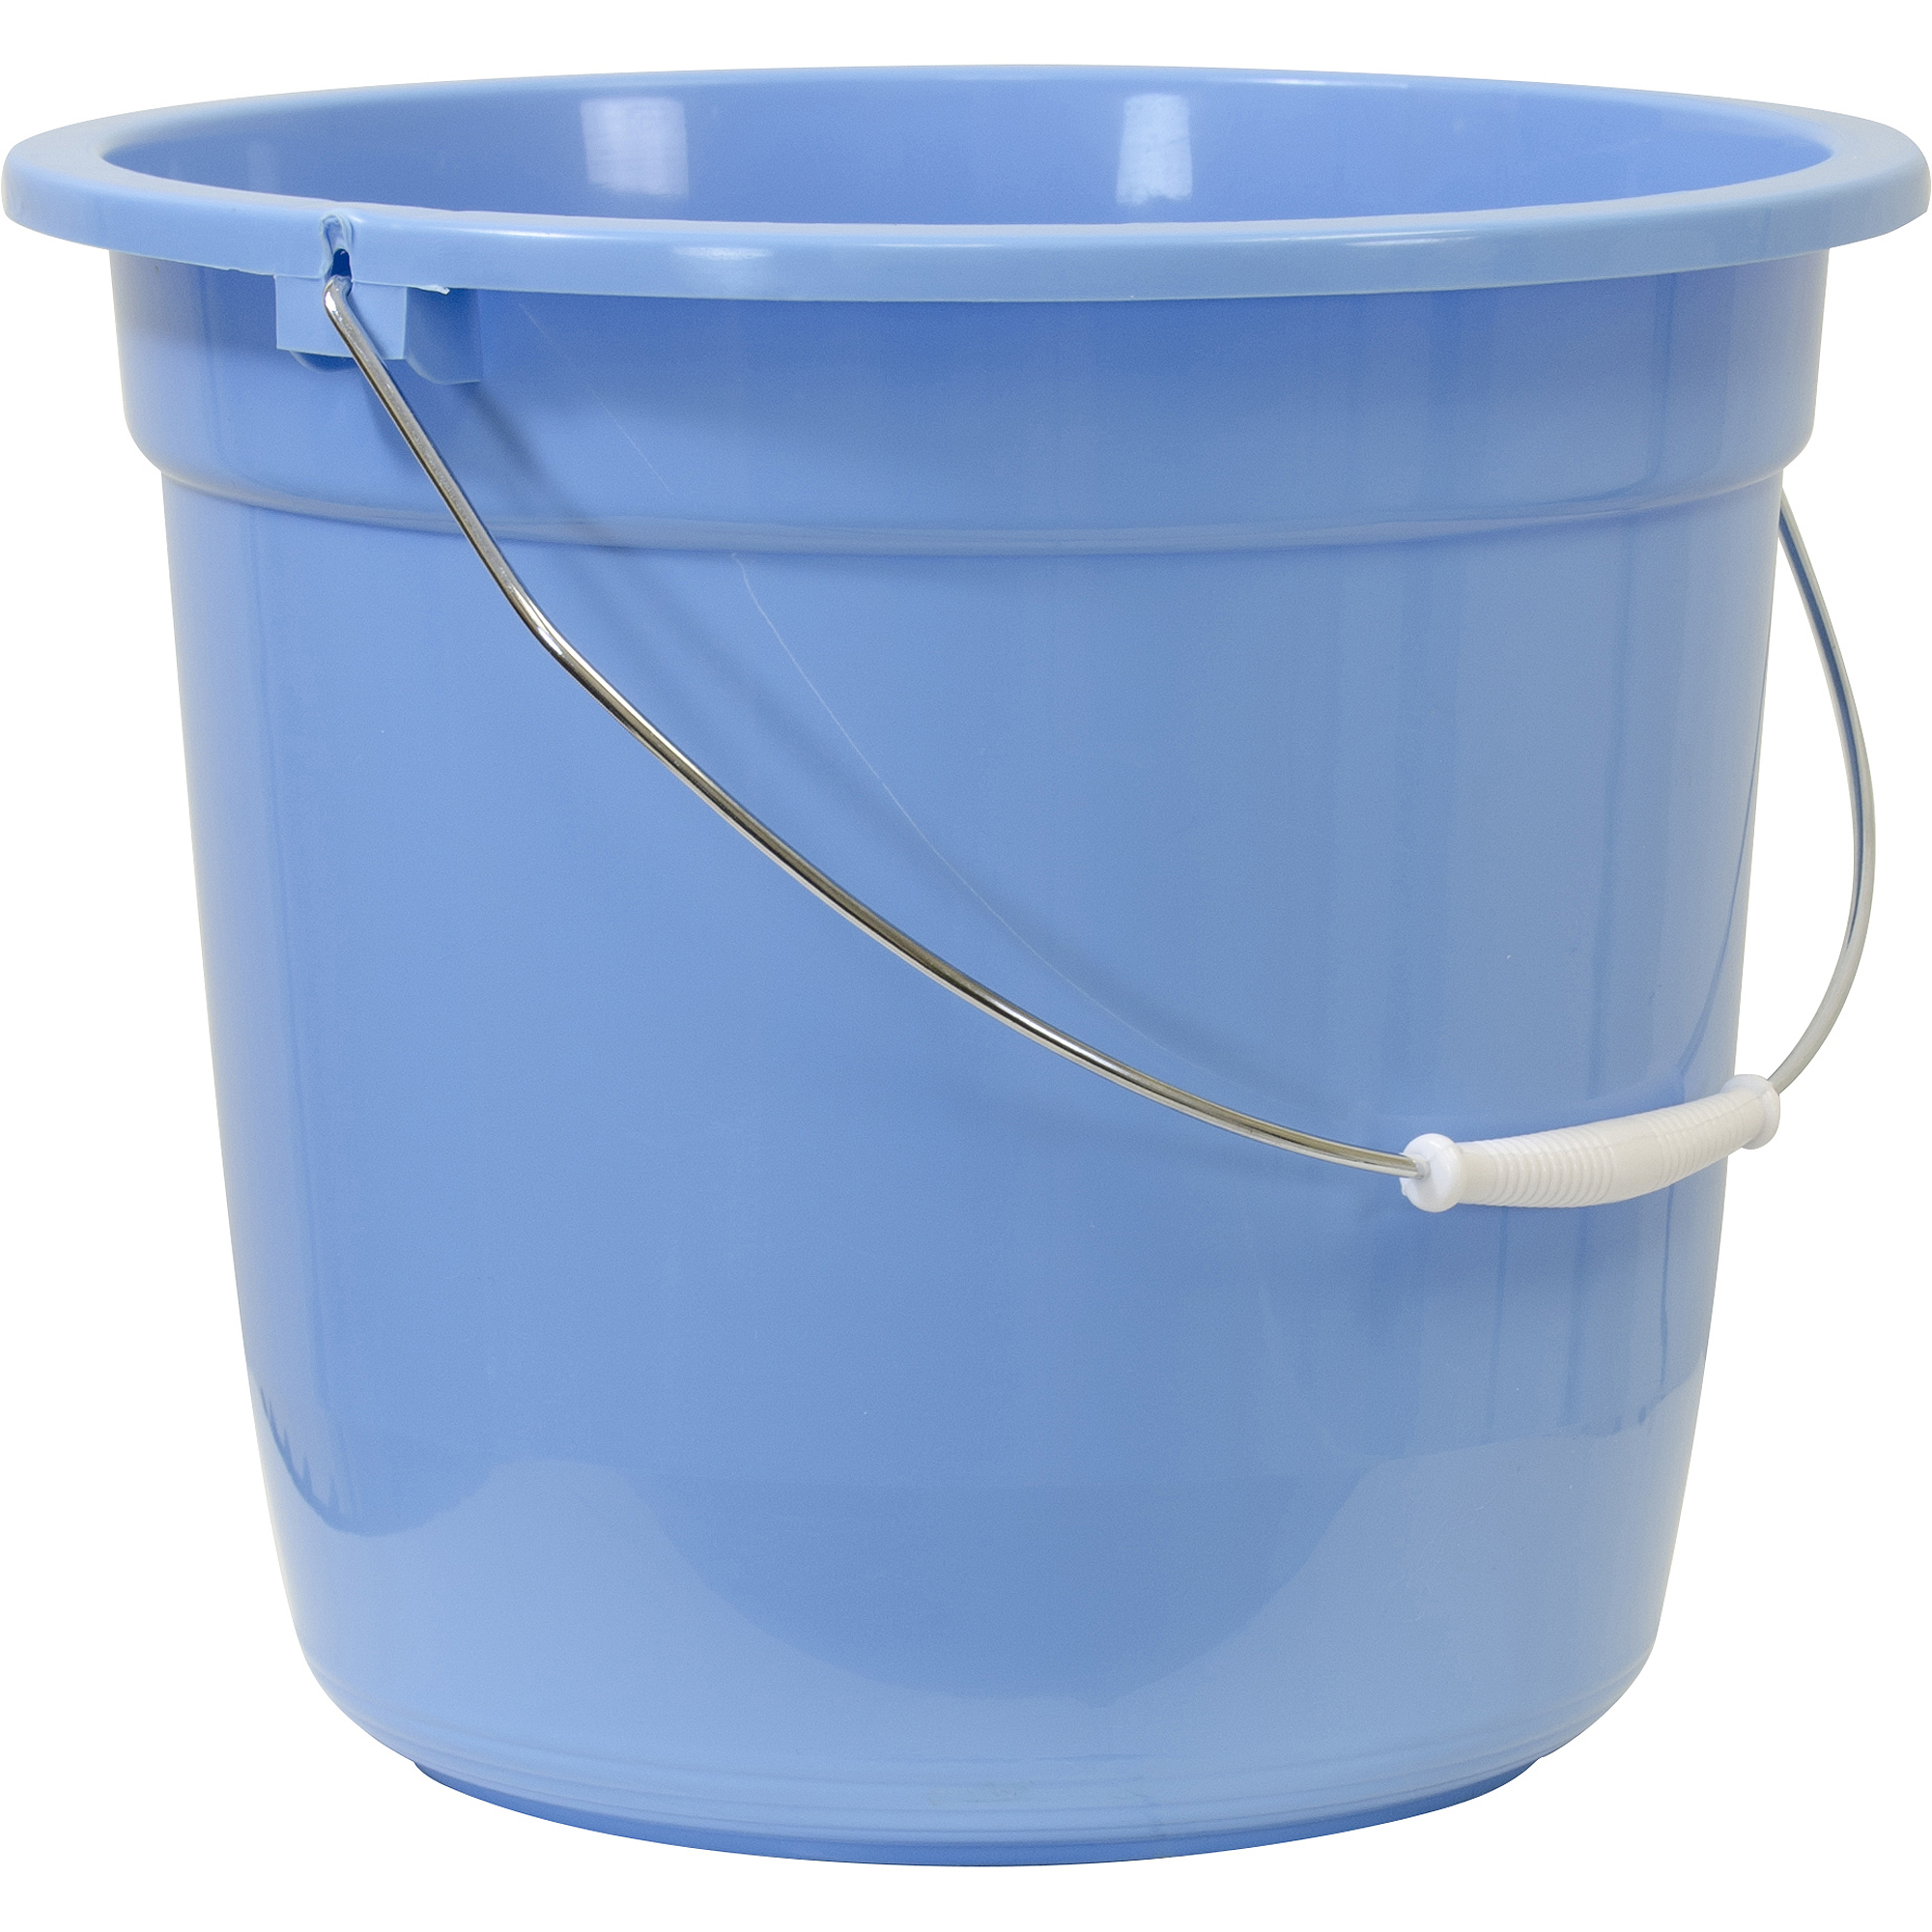
\includegraphics[width=1in]{../images/bucket.jpeg} 
	& 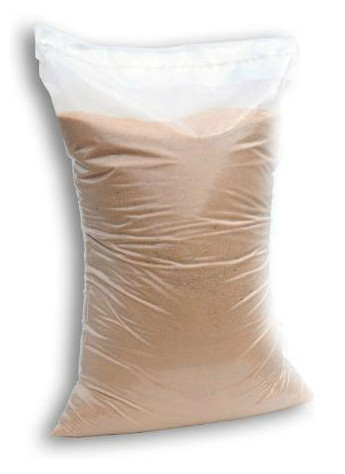
\includegraphics[width = 1in]{../images/sand_bag.jpg} 
	& 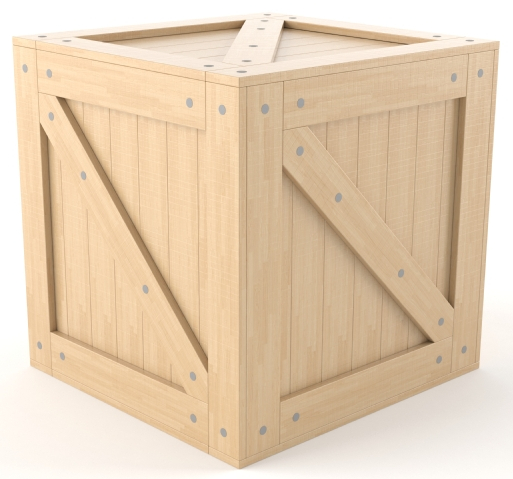
\includegraphics[width=1in]{../images/crate.jpg} \\
	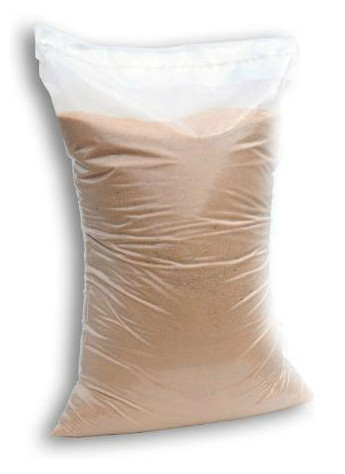
\includegraphics[width=0.2in]{../images/sand_bag.jpg} = 10 $\times$  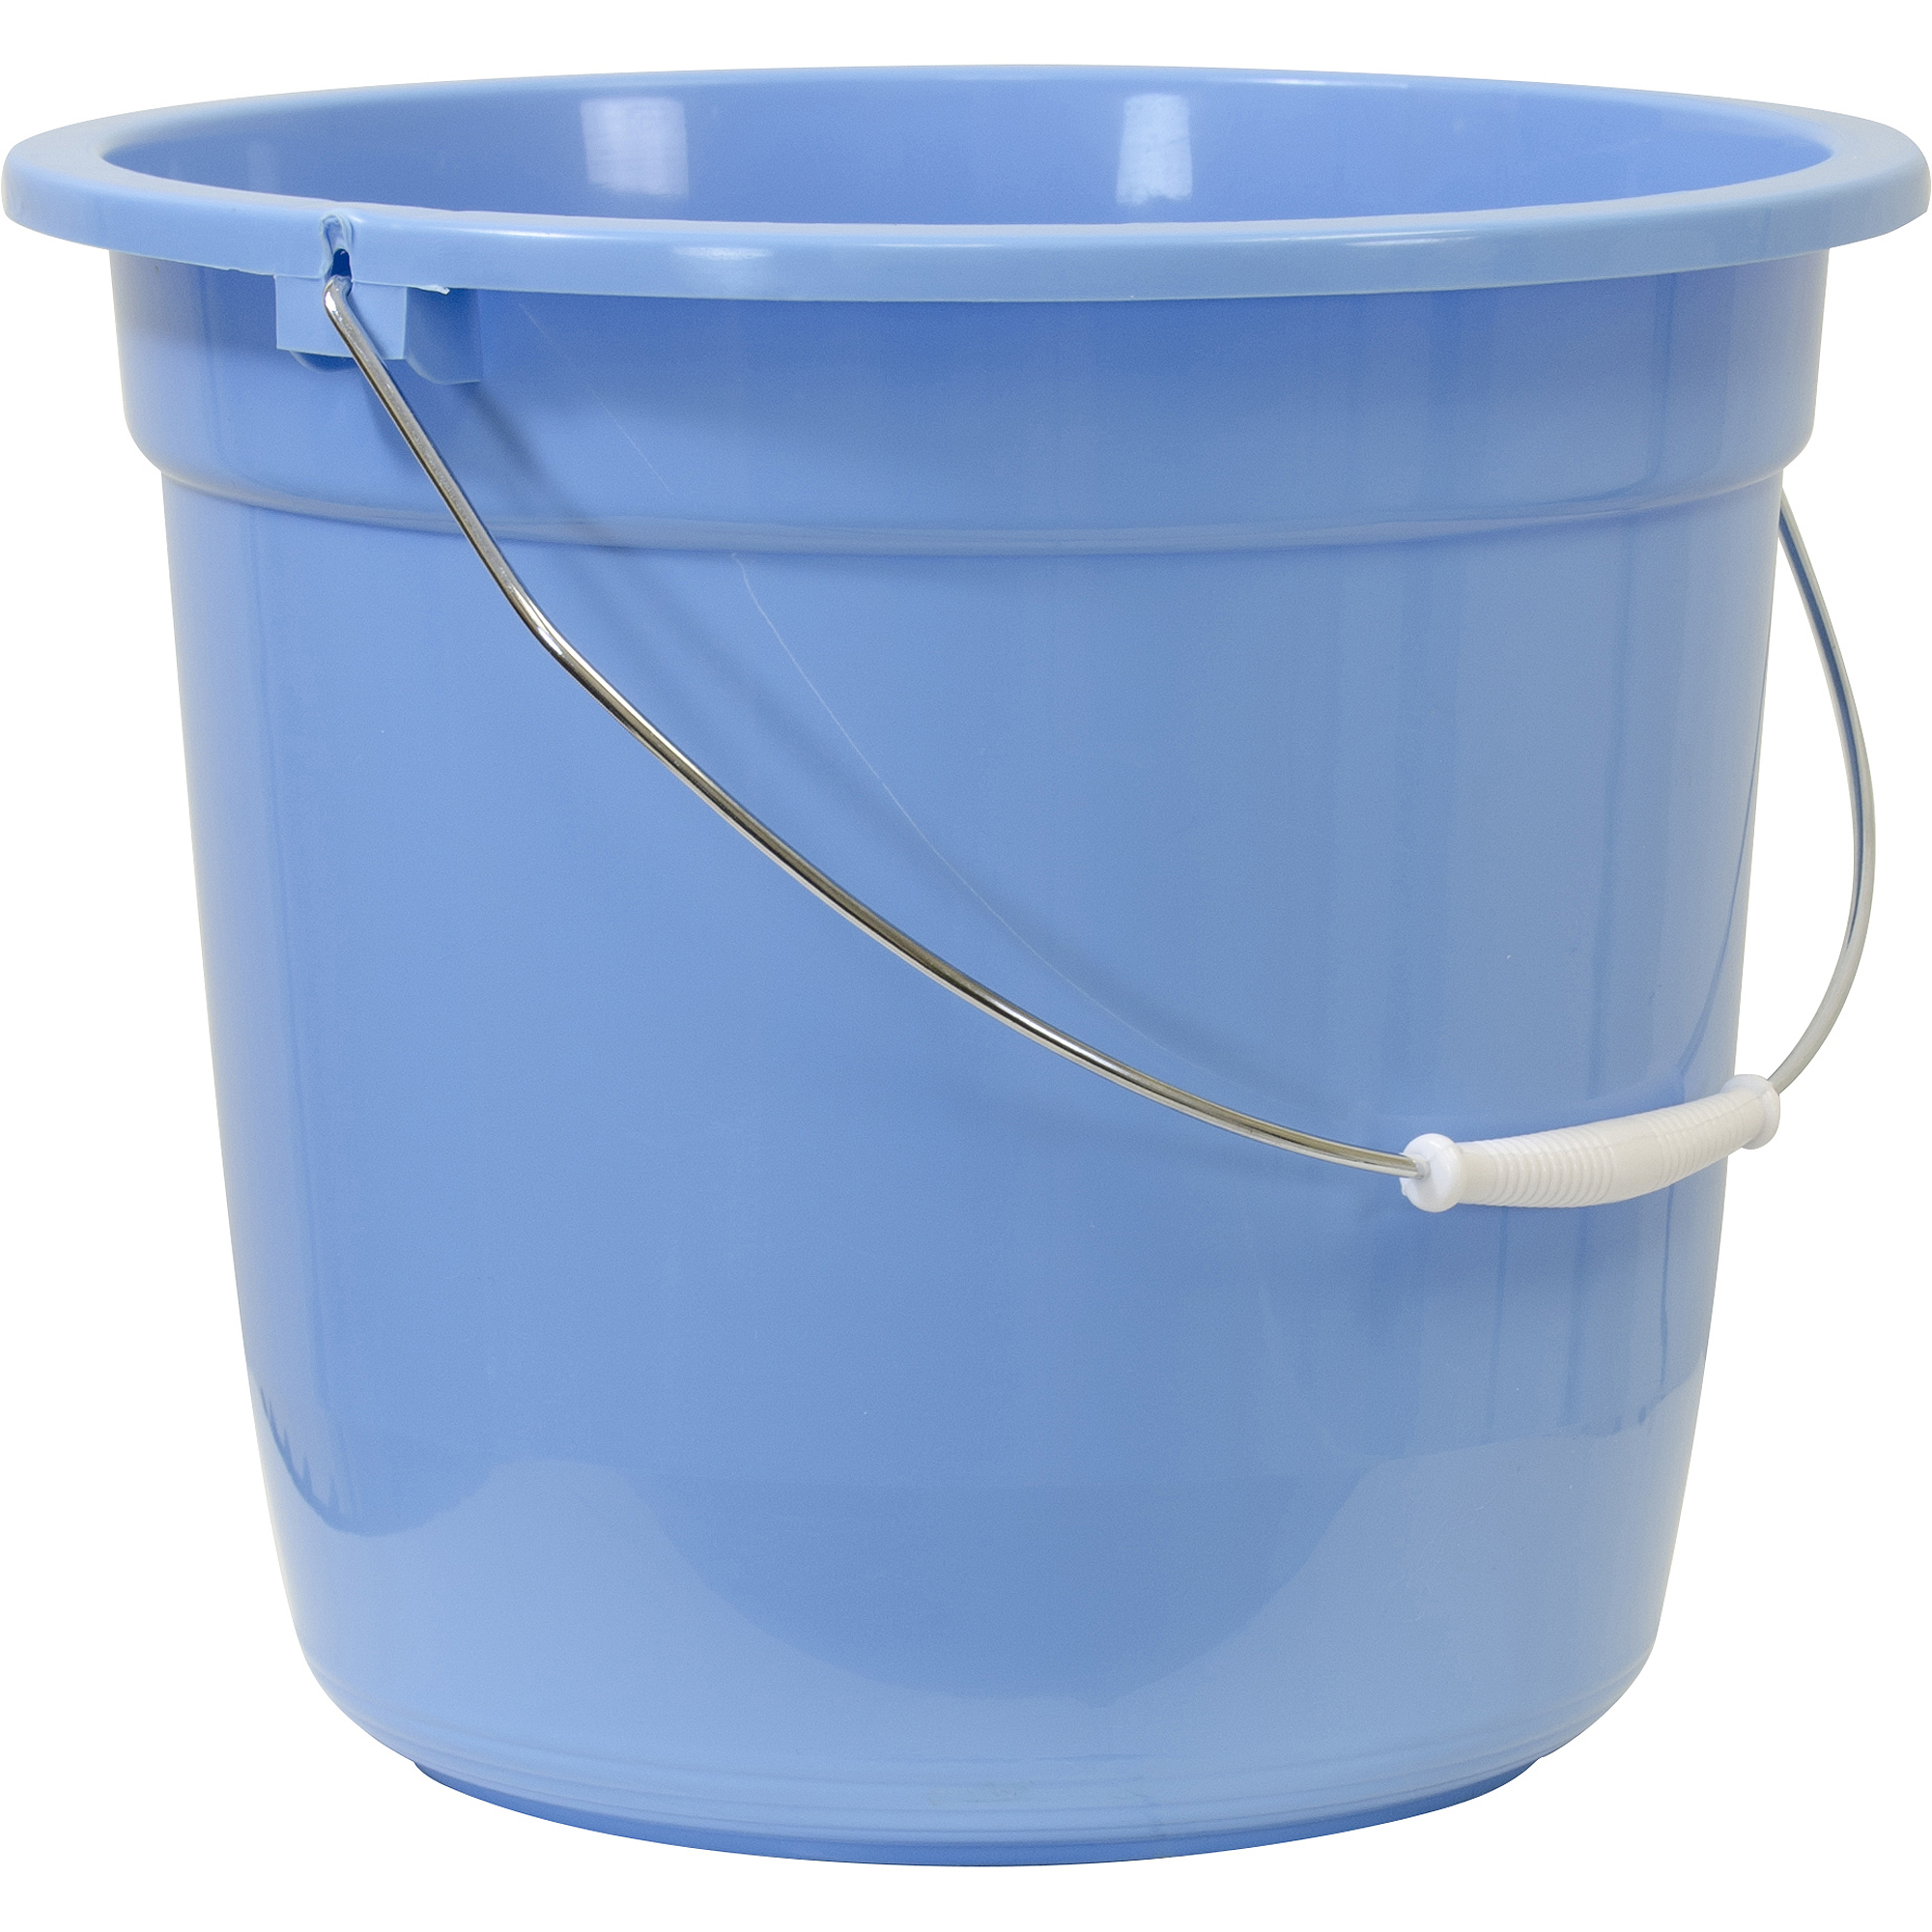
\includegraphics[width = 0.2in]{../images/bucket.jpeg}
	&
	& 10 $\times$  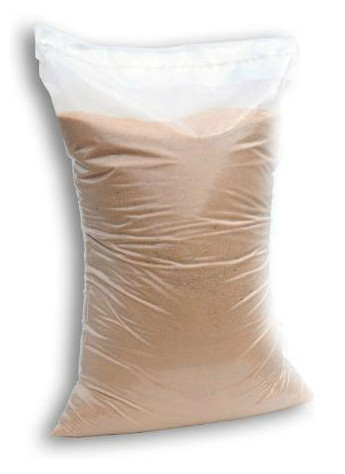
\includegraphics[width = 0.2in]{../images/sand_bag.jpg} = 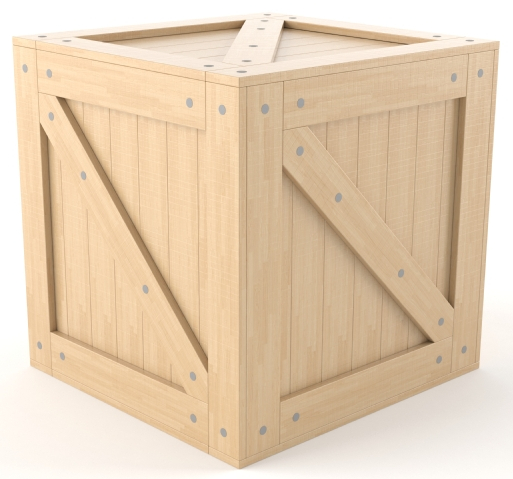
\includegraphics[width=0.21in]{../images/crate.jpg} \\
\end{tabularx}
\vspace{1in}
\begin{parts}
	\item How many buckets does it take to fill 1 crate?
		\vspace{0.4in}
	\item How many buckets can 3 bags be split into?
		\vspace{0.4in}
	\item How many bags will 5 crates fill?
		\vspace{0.4in}
	\item How many bags will 15 buckets fill?
		\vspace{0.4in}
	\item How many crates will 50 buckets fill?
		\vspace{0.4in}
	\item How many buckets can 2.5 crates fill?
		\vspace{0.4in}
		
\clearpage
	\item You compare prices between suppliers.
		\begin{itemize}
			\item Supplier 1 charges 6\$ per bucket.
			\item Supplier 2 charges 70\$ per bag.
			\item Supplier 3 charges 500\$ per crate.
		\end{itemize}
		Which supplier is selling sand the \textit{cheapest}? Which is charging the \textit{most}?
	\vspace{1in}
	\item You discover a fourth supplier, this one selling sand by the \textit{pound}. What do you need to know in order to compare Supplier~1 and Supplier~4?
		\vspace{0.4in}
	\item You weigh 3 bags of sand from Supplier~2, and notice that together they weigh 150~pounds. If Supplier~4 charges 1\$ per pound of sand, then what supplier(s) are they cheaper than, if any?
		\vspace{2in}
\end{parts}

\question
A home owner wishes to re-tile their kitchen, which happens to be a perfect rectangle, measuring 12.0 ft by 14.0 ft. The tiles they are interested in using are square 6.0 inches by 6.0 inches. Ignoring spacing for grout, what is the minimum number of tiles they should buy?
\vspace{2in}

\clearpage
\question
Convert the following into scientific notation (but leave the units the same):
\begin{parts}
	\part 0.020 m
		\vspace{0.4in}
	\part 36 nm
		\vspace{0.4in}
	\part $15.6 \times 10^{6}$ mg
		\vspace{0.4in}
	\part $\frac{4.0 \times 10^{2}~m}{2.0 \times 10^{3}~s}$
		\vspace{1in}
	\part $\frac{4.0\times 10^{-2}~m}{2.0 \times 10^{-3}~s}$
		\vspace{1in}
\end{parts}

\question
Convert the following to cm (useful info: 1 inch $\approx $ 2.5 cm, 1 mile $\approx$ 1.5 km):
\begin{parts}
	\part 100 m
		\vspace{1in}
	\part 15 nm
		\vspace{1in}
	\part 25 km
		\vspace{1in}
	\part 8.0 miles
		\vspace{1in}
	\part 5 inches
		\vspace{1in}
\end{parts}

\question
(Taken from \textit{College Pysics}) Mount Everest, at 29,000 feet, is the tallest mountain on Earth. What is its height in kilometers?
\begin{eqnarray}
	1~m = 3~feet
\end{eqnarray}
	\vspace{1in}

\question 
Olympus Mons is the tallest mountain in the solar system (it is actually a volcano). Its diameter is approximately the size of Arizona, and it stand at 25~km tall. How high is its peek in feet? (Let $1~m = 3~feet$)
\vspace{2in}

\begin{center}Pause here to work on the speed invention activity.\end{center}
\clearpage

\question
(Taken from \textit{College Pysics})The speed limit on many Canadian highways is 100~km/h. Use the conversion factor of
\begin{eqnarray}
	1~miles = 1.5~km
\end{eqnarray}
\begin{parts}
	\part What is this in m/s?
		\vspace{1in}
	\part What is this in miles/hour?
		\vspace{1in}
\end{parts}

\question
You are driving along a highway and pass a mile marker, which reads 81.0. Five minutes later, you pass mile marker 76.0. Assume you neither braked nor accelerated (say, because you are using cruise control).
\begin{parts}
	\part What is your speed in miles/hour?
	\vspace{0.5in}
	\part What is your speed in km/hour?(1 mile = 1.5 km)
	\vspace{0.5in}
\end{parts}

\question
A car is traveling at a speed of 33~m/s.
\begin{parts}
	\part What is its speed in kilometers per hour?
		\vspace{1in}
	\part Is it exceeding the 90~km/h speed limit?
		\vspace{1in}
\end{parts}

\end{questions}

\end{document}

